
\documentclass[landscape]{slides}

%%\usepackage{Sweave}
\newenvironment{thebibliography}{}



\usepackage[coloremph,colorhighlight,LMU,printout]{RSlides}
\usepackage{url,listings}
\usepackage{SweaveSlides}
\usepackage{natbib}

\usepackage[utf8]{inputenc}

\usepackage{hyperref}

../paper/header.tex
\usepackage{amstext}

\setkeys{Gin}{height = 0.9\textheight}

\title{Simultaneous Inference in \\ General Parametric Models}
\author{Torsten Hothorn \\ Institut für Statistik \\ 
(in collaboration with Frank Bretz and \\ Peter Westfall)}
\fancyfoot[L]{\tiny 2008-04-25} %%\copyright{} 2007 Friedrich Leisch
\fancyfoot[R]{\arabic{page}}

\sloppy

\begin{document}

\maketitle

\newslide{Introduction}

\begin{center}
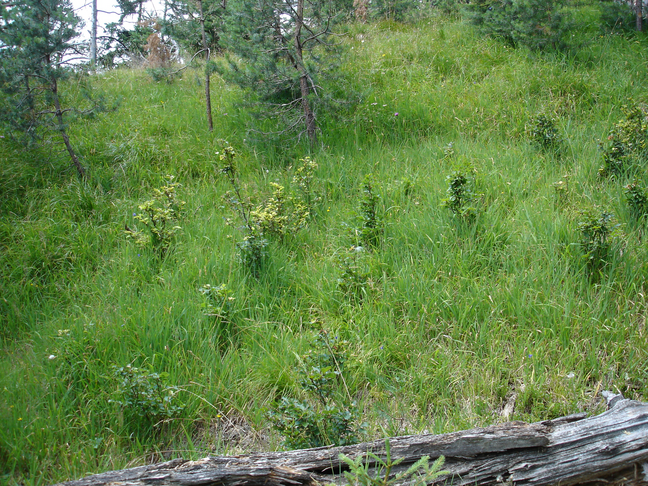
\includegraphics{figs/verbiss}
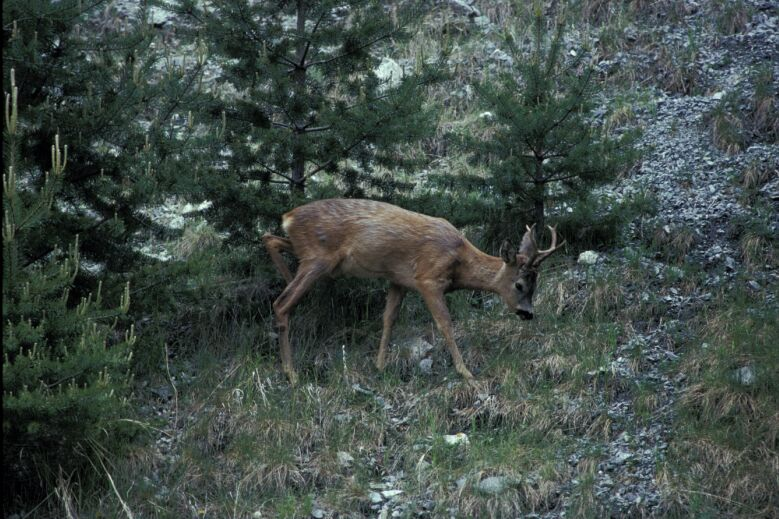
\includegraphics{figs/reh}
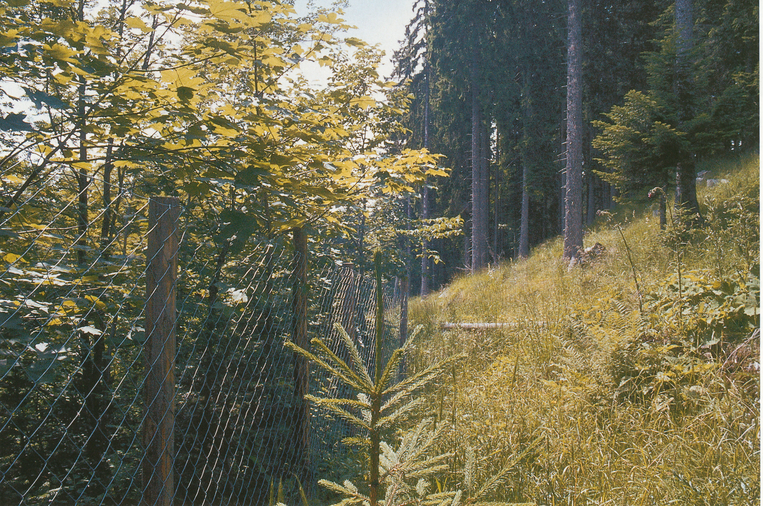
\includegraphics{figs/zaun}
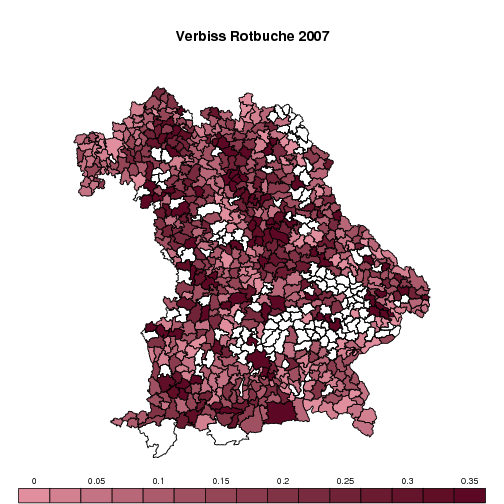
\includegraphics[height=\textheight]{figs/rotbuche2007}
\end{center}

\newslide{Model}

$\M((\Z_1, \dots, \Z_n), \theta, \eta)$ is a (semiparametric) model with

\begin{itemize}
\item $n$ observations $(\Z_1, \dots, \Z_n)$
\item elemental parameters $\theta \in \R^p$ and
\item other (random or nuisance) parameters $\eta$.
\end{itemize}

We are interested in linear functions $\vartheta := \K \theta$ defined
by a constant matrix $\K \in \R^{k, p}$.

\newslide{Estimation}

$\hat{\theta}_n \in \R^p$ is an estimate of $\theta$ and
$\Sraw \in \R^{p,p}$ is an estimate of $\cov(\hat{\theta}_n)$ with
\begin{eqnarray*}
a_n \Sraw \cP \Sigmaraw \in \R^{p,p}
\end{eqnarray*}
for some positive, nondecreasing sequence $a_n$.

A multivariate central limit theorem is assumed:
\begin{eqnarray*}
a_n^{1/2} (\hat{\theta}_n - \theta) \cL \N_p(0, \Sigmaraw).
\end{eqnarray*}

We write $\hat{\theta}_n \an \N_p(\theta, \Sraw)$.

These assumptions are fulfilled for most of the models commonly in use.

\newslide{Distribution of $\vartheta$}

By Theorem 3.3.A in
\cite{Serfling1980}, the linear function $\hat{\vartheta}_n = \K 
\hat{\theta}_n$, i.e., an estimate of our parameters of interest,
also follows an approximate multivariate normal
distribution
\begin{eqnarray*}
\hat{\vartheta}_n = \K \hat{\theta}_n \an \N_k(\vartheta, \SK)
\end{eqnarray*}
with covariance matrix $\SK := \K \Sraw \K^\top$
for any fixed matrix $\K \in \R^{k,p}$

Therefore, we simply assume
\begin{eqnarray*}
\hat{\vartheta}_n \an \N_k(\vartheta, \SK) \text{ with }
a_n \SK \cP \SigmaK := \K \Sigma \K^\top \in \R^{k,k}
\end{eqnarray*}

\newslide{A Statistic and its Distribution}

Consider the multivariate statistic
\begin{eqnarray*}
\T_n := %% \frac{\hat{\vartheta}_n - \vartheta}{\sqrt{\diag(\SK)}} =
\D_n^{-1/2} (\hat{\vartheta}_n - \vartheta) 
%%\an \N_k(0, \Cor_n)
\end{eqnarray*}
where $\D_n = \diag(\SK)$ is the diagonal matrix given by the diagonal elements of
$\SK$.

By Slutzky's Theorem, this statistic is again asymptotically normally
distributed
\begin{eqnarray*}
\T_n \an \N_k(0, \Cor_n)
\end{eqnarray*}
where
\begin{eqnarray*}
\Cor_n = \D_n^{-1/2} \SK \D_n^{-1/2} \in \R^{k,k}
\end{eqnarray*}
is the correlation matrix of the $k$-dimensional statistic $\T_n$. 


\newslide{General Linear Hypothesis}

Consider the null hypothesis
\begin{eqnarray*}
H_0: \vartheta := \K \theta = \m.
\end{eqnarray*}

Classically, $F$- or $\chi^2$-statistics are used to test $H_0$.
However, a rejection of $H_0$ 
does not give further indication about the nature of the significant
result. Therefore, one is often interested in the individual null hypotheses
\begin{eqnarray*}
H_0^j: \vartheta_j = \m_j.
\end{eqnarray*}

Testing the hypotheses set $\{H_0^1, \ldots, H_0^k\}$ simultaneously thus requires the individual
assessments while maintaining the familywise error rate.

\newslide{A Maximum-Type Statistic}

An alternative test statistic for testing $H_0$ is
\begin{eqnarray*}
\max(|\T_n|)
\end{eqnarray*}

Can we approximate it's distribution under $H_0$ efficiently?

We have to find a good approximation of $\Prob(\max(|\T_n|) \le t)$
for some $t \in \R^+$.

\newslide{Null-Distribution and a Global Test}

\begin{eqnarray*}
\Prob(\max(|\T_n|) \le t) = \int\limits_{-t}^t \cdots \int\limits_{-t}^t
\varphi_k(x_1, \dots, x_k; \Cor) \, dx_1 \cdots dx_k =: g(\Cor, t) 
\end{eqnarray*}
where $\varphi_k$ is the $k$-dimensional normal density function.

$\Cor$ is not known but $g(\Cor, t)$ is a continuous function of $\Cor$ 
and converges as $\Cor_n \cP \Cor$. The integral can be approximated
by quasi-randomized Monte-Carlo methods \citep{Genz1992,GenzBretz1999}.

The resulting global $p$-value 
for $H_0$ is then 
\begin{eqnarray*}
p_\text{global} = 1 - g(\Cor_n, \max|\tt|)
\end{eqnarray*}
when $\T = \tt$ has been observed.

\newslide{Simultaneous Inference}

But what about the partial hypotheses $H_0^1, \ldots, H_0^k$?

It's simple!

The multiplicity adjusted $p$-value for the $j$th
individual two-sided hypothesis 
\begin{eqnarray*}
H_0^j: \vartheta_j = \m_j, j = 1, \dots, k,
\end{eqnarray*}
is given by 
\begin{eqnarray*}
p_j = 1 - g(\Cor_n, |t_j|),
\end{eqnarray*}
where $t_1, \dots, t_k$ denote the observed test statistics (single-step procedure).

Reject each $H_0^j$ at family-wise error rate $\alpha$ when $p_j \leq \alpha$.

\newslide{Simultenous Confidence Intervals}

A simultaneous $(1 - 2\alpha)
\times 100\%$ confidence interval for $\vartheta$ is given by 
\begin{eqnarray*}
\hat{\vartheta}_n \pm q_\alpha \D_n^{1/2}
\end{eqnarray*}
where $q_\alpha$ is the (approximate) $1 - \alpha$ quantile of the distribution of $\T_n$.

\newslide{Examples: Linear Regression}

Observations $\Z_i = (Y_i, \X_i), i = 1, \dots, n$ consist of a response $Y_i$
and exploratory variables $\X_i = (X_{i1}, \dots, X_{iq})$.

Model:
\begin{eqnarray*}
Y_i = \beta_0 + \sum_{j = 1}^q \beta_j X_{ij} + \sigma \varepsilon_i,
\end{eqnarray*}
with elemental parameters $\theta = (\beta_0, \beta_1, \dots, \beta_q)$
estimated via
\begin{eqnarray*}
\hat{\theta}_n = \left(\X^\top\X\right)^{-1} \X^\top \Y \sim \N%
_{q+1}\left(\theta, \sigma^2 \left(\X^\top\X\right)^{-1}\right),
\end{eqnarray*}

Now
\begin{eqnarray*}
\hat{\vartheta}_n = \K \hat{\theta}_n \sim \N_k(\K \theta, \sigma^2 \K \left(\X^\top\X%
\right)^{-1} \K^\top)
\end{eqnarray*}
and
\begin{eqnarray*}
\T_n = \D_n^{-1/2} \hat{\vartheta}_n \sim t_{q+1}(n - q, \Cor),
\end{eqnarray*}
(Note: the normal density $\varphi_k$ can be replaced by the
$t$-density in this case!)

\newslide{Predicting Body Fat}

\cite{garcia2005} describe a linear model
for total body fat prediction.

\textbf{Aim:} Based on $p = 9$ simple measurements (circumferences of elbow, knee etc)
we want to estimate a simple (!) formula to predict the total body fat obtained for
$n = 71$ healthy German women by means of Dual Energy X-Ray Absorptiometry. 

\textbf{Problem:} Variable selection!

\newslide{Linear Model Fit}

\begin{Schunk}
\begin{Sinput}
R> data("bodyfat", package = "mboost")
R> lmod <- lm(DEXfat ~ ., data = bodyfat)
R> summary(lmod)
\end{Sinput}
\end{Schunk}
\begin{Schunk}
\begin{Soutput}
               Estimate Std. Error t value  Pr(>|t|)    
(Intercept)  -69.028276   7.516860 -9.1831 4.184e-13 ***
age            0.019962   0.032213  0.6197  0.537767    
waistcirc      0.210487   0.067145  3.1348  0.002644 ** 
hipcirc        0.343513   0.080373  4.2740 6.852e-05 ***
elbowbreadth  -0.412369   1.022907 -0.4031  0.688259    
kneebreadth    1.757984   0.724952  2.4250  0.018286 *  
anthro3a       5.742295   5.207524  1.1027  0.274492    
anthro3b       9.866431   5.657864  1.7438  0.086224 .  
anthro3c       0.387430   2.087463  0.1856  0.853376    
anthro4       -6.574395   6.489177 -1.0131  0.314999    
---
Signif. codes:  0 ‘***’ 0.001 ‘**’ 0.01 ‘*’ 0.05 ‘.’ 0.1 ‘ ’ 1 
\end{Soutput}
\end{Schunk}


\newslide{Parameters of Interest}

\begin{Schunk}
\begin{Sinput}
R> K <- cbind(0, diag(length(coef(lmod)) - 1))
R> rownames(K) <- names(coef(lmod))[-1]
R> lmod_glht <- glht(lmod, linfct = K) 
R> K
\end{Sinput}
\begin{Soutput}
             [,1] [,2] [,3] [,4] [,5] [,6] [,7] [,8] [,9] [,10]
age             0    1    0    0    0    0    0    0    0     0
waistcirc       0    0    1    0    0    0    0    0    0     0
hipcirc         0    0    0    1    0    0    0    0    0     0
elbowbreadth    0    0    0    0    1    0    0    0    0     0
kneebreadth     0    0    0    0    0    1    0    0    0     0
anthro3a        0    0    0    0    0    0    1    0    0     0
anthro3b        0    0    0    0    0    0    0    1    0     0
anthro3c        0    0    0    0    0    0    0    0    1     0
anthro4         0    0    0    0    0    0    0    0    0     1
\end{Soutput}
\end{Schunk}

\newslide{$F$-Test}

\begin{Schunk}
\begin{Sinput}
R> summary(lmod_glht, test = Ftest())
\end{Sinput}
\begin{Soutput}
	 General Linear Hypotheses

Linear Hypotheses:
                  Estimate
age == 0           0.01996
waistcirc == 0     0.21049
hipcirc == 0       0.34351
elbowbreadth == 0 -0.41237
kneebreadth == 0   1.75798
anthro3a == 0      5.74230
anthro3b == 0      9.86643
anthro3c == 0      0.38743
anthro4 == 0      -6.57439

Global Test:
      F DF1 DF2    Pr(>F)
1 81.35   9  61 1.387e-30
\end{Soutput}
\end{Schunk}

\newslide{Maximum Test}
\begin{Schunk}
\begin{Sinput}
R> summary(lmod_glht)
\end{Sinput}
\begin{Soutput}
	 Simultaneous Tests for General Linear Hypotheses

Fit: lm(formula = DEXfat ~ ., data = bodyfat)

Linear Hypotheses:
                  Estimate Std. Error t value p value    
age == 0           0.01996    0.03221   0.620  0.9959    
waistcirc == 0     0.21049    0.06714   3.135  0.0213 *  
hipcirc == 0       0.34351    0.08037   4.274  <0.001 ***
elbowbreadth == 0 -0.41237    1.02291  -0.403  0.9998    
kneebreadth == 0   1.75798    0.72495   2.425  0.1316    
anthro3a == 0      5.74230    5.20752   1.103  0.8948    
anthro3b == 0      9.86643    5.65786   1.744  0.4783    
anthro3c == 0      0.38743    2.08746   0.186  1.0000    
anthro4 == 0      -6.57439    6.48918  -1.013  0.9295    
---
Signif. codes:  0 ‘***’ 0.001 ‘**’ 0.01 ‘*’ 0.05 ‘.’ 0.1 ‘ ’ 1 
(Adjusted p values reported -- single-step method)
\end{Soutput}
\end{Schunk}

\newslide{ANOVA}

Model:
\begin{eqnarray*}
Y_{ij} = \mu + \gamma_{j} + \varepsilon_{ij}
\end{eqnarray*}

Overparameterized, usually the elemental parameters are
$theta = (\mu, \gamma_2 - \gamma_1, \gamma_3 - \gamma_1, \dots, \gamma_q - \gamma_1)$.

\textbf{Dunnett many-to-one comparisons}:
\begin{eqnarray*}
\K_\text{Dunnett} &=& (0, \diag(q)) \\
\vartheta_\text{Dunnett} &=& \K_\text{Dunnett} \theta = (\gamma_2 - \gamma_1, \gamma_3 - \gamma_1,
\dots, \gamma_q - \gamma_1)
\end{eqnarray*}

\textbf{Tukey all-pair comparisons}:
\begin{eqnarray*}
\K_\text{Tukey} &=& \left(
\begin{array}{rrr}
0 & 1 & 0 \\ 
0 & 0 & 1 \\ 
0 & 1 & -1%  
\end{array}  
\right) \\
\vartheta_\text{Tukey} &=& \K_\text{Tukey} \theta = (\gamma_2 - \gamma_1, \gamma_3 - \gamma_1,
\gamma_2 - \gamma_3).
\end{eqnarray*}

\newslide{Genetic Components of Alcoholism}

\begin{center}   
\includegraphics{generalsiminf-alpha-data-figure}
\end{center}

\newpage

\begin{Schunk}
\begin{Sinput}
R> data("alpha", package = "coin")   
R> amod <- aov(elevel ~ alength, data = alpha)
R> confint(glht(amod, linfct = mcp(alength = "Tukey")))
\end{Sinput}
\begin{Soutput}
	 Simultaneous Confidence Intervals

Multiple Comparisons of Means: Tukey Contrasts


Fit: aov(formula = elevel ~ alength, data = alpha)

Estimated Quantile = 2.3716
95% family-wise confidence level
 

Linear Hypotheses:
                          Estimate lwr      upr     
intermediate - short == 0  0.43415 -0.47569  1.34399
long - short == 0          1.18875 -0.04509  2.42259
long - intermediate == 0   0.75460 -0.33128  1.84047
\end{Soutput}
\end{Schunk}

\newpage

\begin{Schunk}
\begin{Sinput}
R> amod_glht_sw <- glht(amod, linfct = mcp(alength = "Tukey"),
+                       vcov = sandwich)
R> confint(amod_glht_sw)
\end{Sinput}
\begin{Soutput}
	 Simultaneous Confidence Intervals

Multiple Comparisons of Means: Tukey Contrasts


Fit: aov(formula = elevel ~ alength, data = alpha)

Estimated Quantile = 2.372
95% family-wise confidence level
 

Linear Hypotheses:
                          Estimate   lwr        upr       
intermediate - short == 0  0.4341523 -0.5714214  1.4397260
long - short == 0          1.1887500  0.1375775  2.2399225
long - intermediate == 0   0.7545977 -0.0005637  1.5097591
\end{Soutput}
\end{Schunk}

\newpage

\setkeys{Gin}{height = 0.6\textheight}
\begin{center}
\includegraphics{generalsiminf-alpha-confint-plot}
\end{center}  

\newslide{Generalized Mixed Models}

Model:
\begin{eqnarray*}
\E(\mathbf{y}_i) = h(\mathbf{X}_i \theta + \mathbf{Z} \mathbf{b}_i)
\end{eqnarray*}
for the $n_i$ observations in group $i$ with random effects $\mathbf{b}_i$.

We are interested in inference about $\K \theta$. For example in a logistic mixed model, in
confidence intervals for the predicted probabilities
\begin{eqnarray*}
\left(\left(1 + \exp\left(- \left(\hat{\vartheta}_n - q_\alpha \D_n^{1/2}\right)\right)\right)^{-1},
\left(1 + \exp\left(- \left(\hat{\vartheta}_n + q_\alpha \D_n^{1/2}\right)\right)\right)^{-1}\right).
\end{eqnarray*}

\newslide{Dear Browsing in Frankonia}



\begin{Schunk}
\begin{Sinput}
R> mmod <- lmer(damage ~ species - 1 + (1 | lattice / plot),
+               data = trees513, family = binomial())
R> K <- diag(length(fixef(mmod)))
\end{Sinput}
\end{Schunk}


\begin{Schunk}
\begin{Sinput}
R> ci <- confint(glht(mmod, linfct = K))
R> ci$confint <- 1 - binomial()$linkinv(ci$confint)
R> ci$confint[,2:3] <- ci$confint[,3:2]
R> ci
\end{Sinput}
\begin{Soutput}
	 Simultaneous Confidence Intervals

Fit: NULL

Estimated Quantile = 2.6069
95% family-wise confidence level
 

Linear Hypotheses:
                             Estimate  lwr       upr      
spruce (119) == 0            0.0054694 0.0006618 0.0436751
pine (823) == 0              0.0087108 0.0032325 0.0232569
beech (266) == 0             0.0668613 0.0291410 0.1460614
oak (1258) == 0              0.2173645 0.1370886 0.3268432
ash/maple/elm/lime (30) == 0 0.2240237 0.0382194 0.6771497
hardwood (other) (191) == 0  0.1697274 0.0883524 0.3012820
\end{Soutput}
\end{Schunk}

\setkeys{Gin}{height = 0.9\textheight}

\begin{center}
\includegraphics{generalsiminf-trees-plot}
\end{center}

%%\bibliography{../paper/references}
%%\bibliographystyle{plainnat}


\end{document}

